\section{Charakterisierung des Messaufbaus}
\subsection{Durchführung}
\label{sect:durchführung}
\subsubsection*{P-I-Kennlinie der Laserdiode}
Für die erste Messung werden nur die beiden Linsen im Strahlengang justiert, alle anderen Elemente sind entfernt.
Das Peltierelement wird auf 33.9$^\circ$C eingestellt und die Spannung an der
Photodiode bei verschiedenen Laserdiodenströmen aufgezeichnet.

\subsubsection*{Temperaturabhängigkeit der Laserfrequenz}
Zur Bestimmung der Temperaturabhängigkeit der
Laserfrequenz wird das Etalon in den Strahlengang eingesetzt und der Diodenstrom mit einem Dreiecksignal moduliert
(Signalgenerator ist das im Aufbau vorhandene Netzgerät).
Der Konstantanteil des Stroms beträgt 63.6\,mA.
Modulationssignal und Photodiodensignal werden mit dem Oszilloskop gemessen und die Wanderung eines Etalonpeaks
im Temperaturbereich von 32.6$^\circ$C bis 33.7$^\circ$C beobachtet.

\subsubsection*{Zeitabhängigkeit der Laserfrequenz}
Der Aufbau zur Bestimmung der Stromabhängigkeit ist
wie bei der Messung der Temperaturabhängigkeit.
Der Konstantanteil des Laserstroms beträgt bei der Messung 64.7\,mA,
die Temperatur der Laserdiode 34.0$^\circ$C.
Die Modulation des Laserstroms findet mit dem \emph{instec function~generator GFG-8210} statt,
da dieser eine bessere Signalqualität als das Netzgerät des Versuchsaufbaus liefert.
Die Frequenz des Modulationssignals beträgt 0.1\,kHz, seine Amplitude 0.7\,V.

\subsection{Auswertung}
\subsubsection*{P-I-Kennlinie der Laserdiode}
\begin{figure}[H]
    \begin{center}
        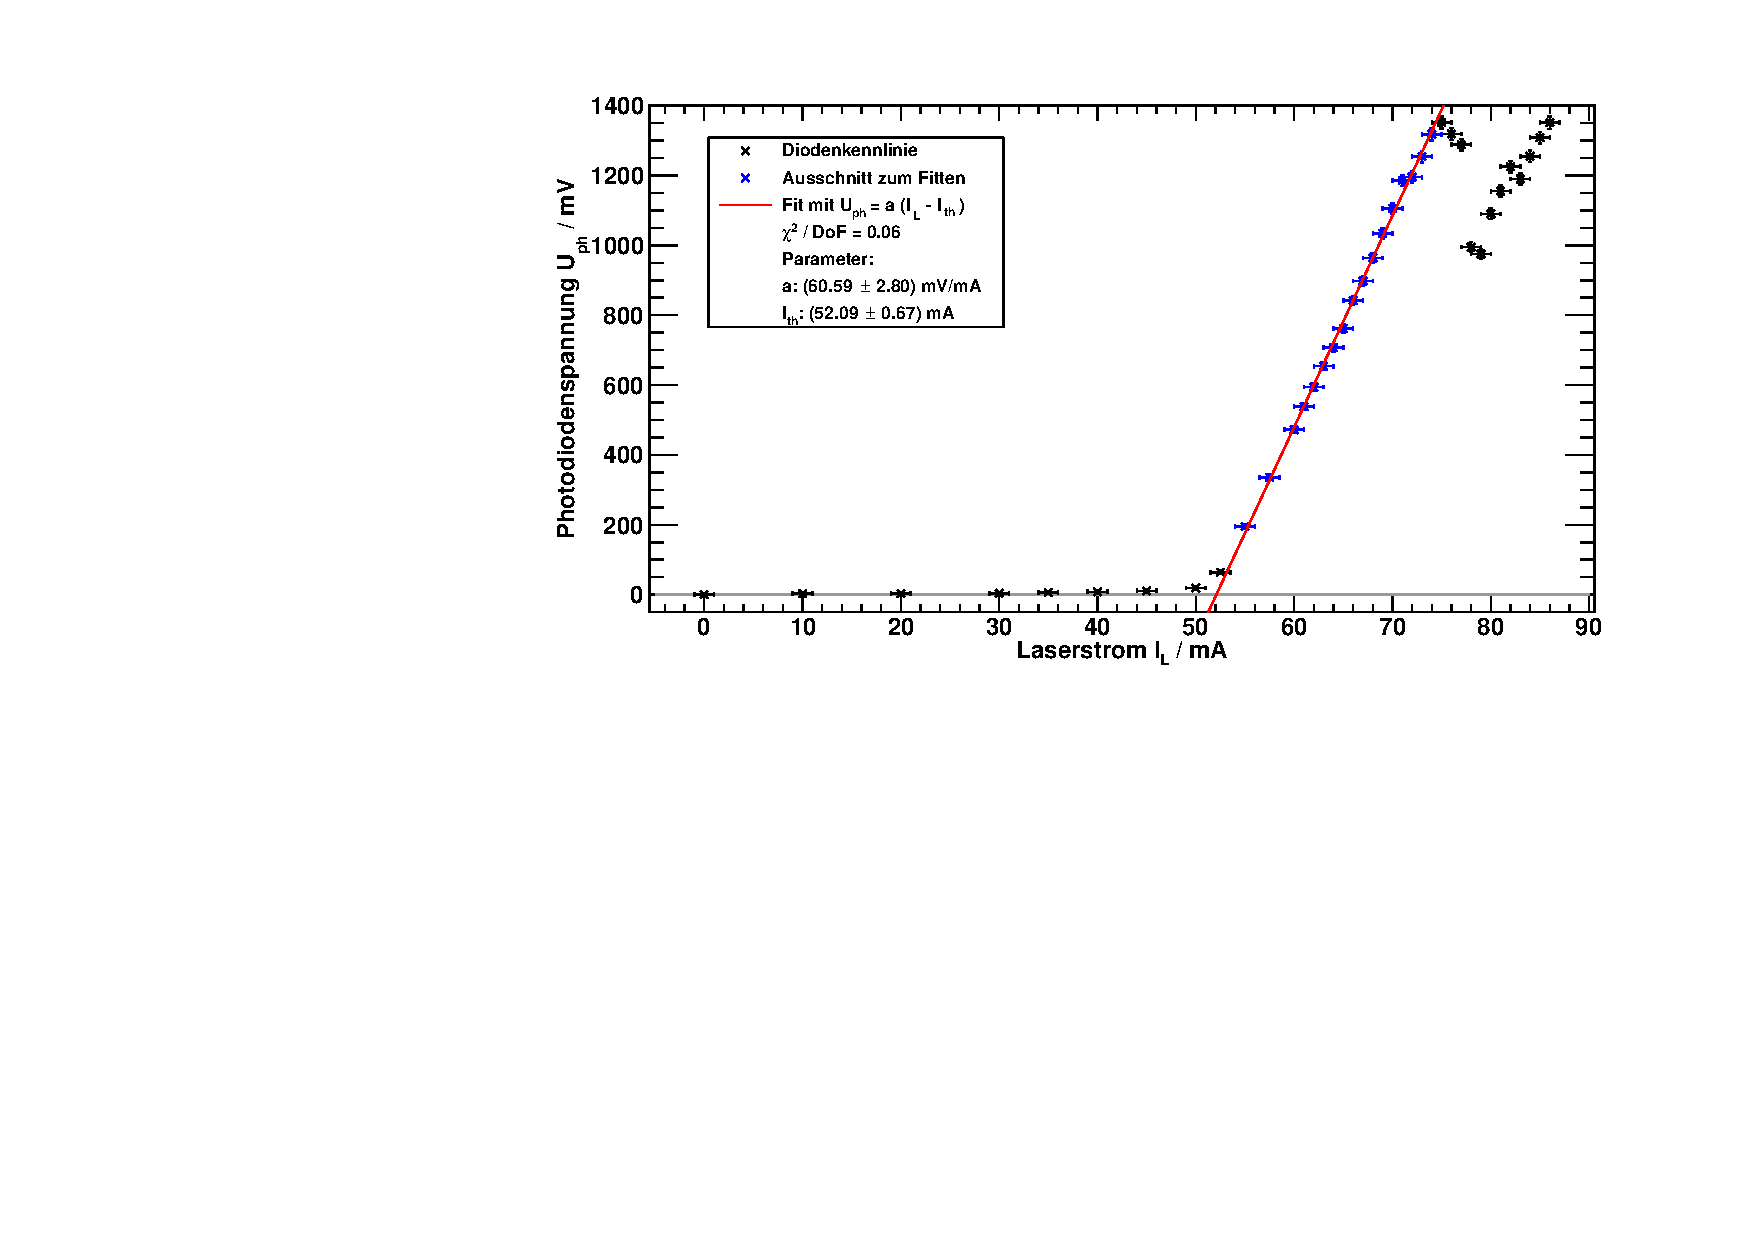
\includegraphics[width=\textwidth]{../img/part1/diodenkennlinie.pdf}
        \caption{$P$-$I$-Kennlinie der Laserdiode: Abhängigkeit der Spannung
        an der Photodiode vom Laserstrom. Man erkennt den linearen Arbeitsbereich (gefitteter Teil),
        in dem ein modensprungfreier Betrieb möglich ist.}
        \label{img:Kennlinie}
    \end{center}
\end{figure}
\autoref{img:Kennlinie} zeigt die $P$-$I$-Kennlinie der Photodiode.
Als Fehler auf die Photodiodenspannung wurde ein Fehler von
\begin{equation}
    s_{U_{\text{ph}}}= 5\,\text{mV} + 0.01 \cdot U_{\text{ph}}
\end{equation}
angenommen.
Der Fehler auf den Strom $s_{I_{\text{L}}}$ beträgt ein Digit vom Lasernetzgerät:
\begin{equation}
    s_{I_{\text{L}}} = 0.1\,\text{mA} \ \, .
\end{equation}
Alle Messwerte wurden um den Spannungsoffset bei $I_{\text{L}}$=0\,mA verschoben.
Ein linearer Fit des modensprungfreien Laserbereichs zwischen 55\,mA und 71\,mA
liefert eine Laserschwelle $I_{\text{th}}$ von
\begin{equation}
    I_{\text{th}}=(52.01 \pm 0.13)\,\text{mA} \ \, .
\end{equation}